% SETUP
\documentclass[11pt]{article}
\linespread{1.1}
\usepackage[utf8]{inputenc}
\usepackage{graphicx, amsmath, array, graphics, amssymb, epsfig, psfrag, geometry, alltt, subfiles, blindtext, pdfpages, mathtools, float, multirow}
\usepackage[export]{adjustbox}
\usepackage{fancyhdr}
\usepackage{array}
\usepackage{hyperref}

%%%%%%%%%%%%%%  code listing
\usepackage{listings}
\usepackage{color} %red, green, blue, yellow, cyan, magenta, black, white
\definecolor{mygreen}{RGB}{2,94,33} % color values Red, Green, Blue
\definecolor{mylilas}{RGB}{170,55,241}

\lstset{language=Matlab,%
    %basicstyle=\color{red},
    breaklines=true,%
    morekeywords={matlab2tikz},
    keywordstyle=\color{blue},%
    morekeywords=[2]{1}, keywordstyle=[2]{\color{black}},
    identifierstyle=\color{black},%
    stringstyle=\color{mylilas},
    commentstyle=\color{mygreen},%
    showstringspaces=false,%without this there will be a symbol in the places where there is a space
    numbers=left,%
    numberstyle={\tiny \color{black}},% size of the numbers
    numbersep=9pt, % this defines how far the numbers are from the text
    emph=[1]{for,end,break},emphstyle=[1]\color{black}, %some words to emphasise
    %emph=[2]{word1,word2}, emphstyle=[2]{style},    
}

\geometry{a4paper, top = 20mm, bottom = 20mm, left = 15mm, right = 15mm}
\DeclarePairedDelimiter\set\{\}

% Headers
\pagestyle{fancy}
\fancyhf{}
\chead{ELEN90064 Advanced Control Systems - Workshop 4 Report}
\cfoot{\thepage}

\begin{document}
% Cover Sheet
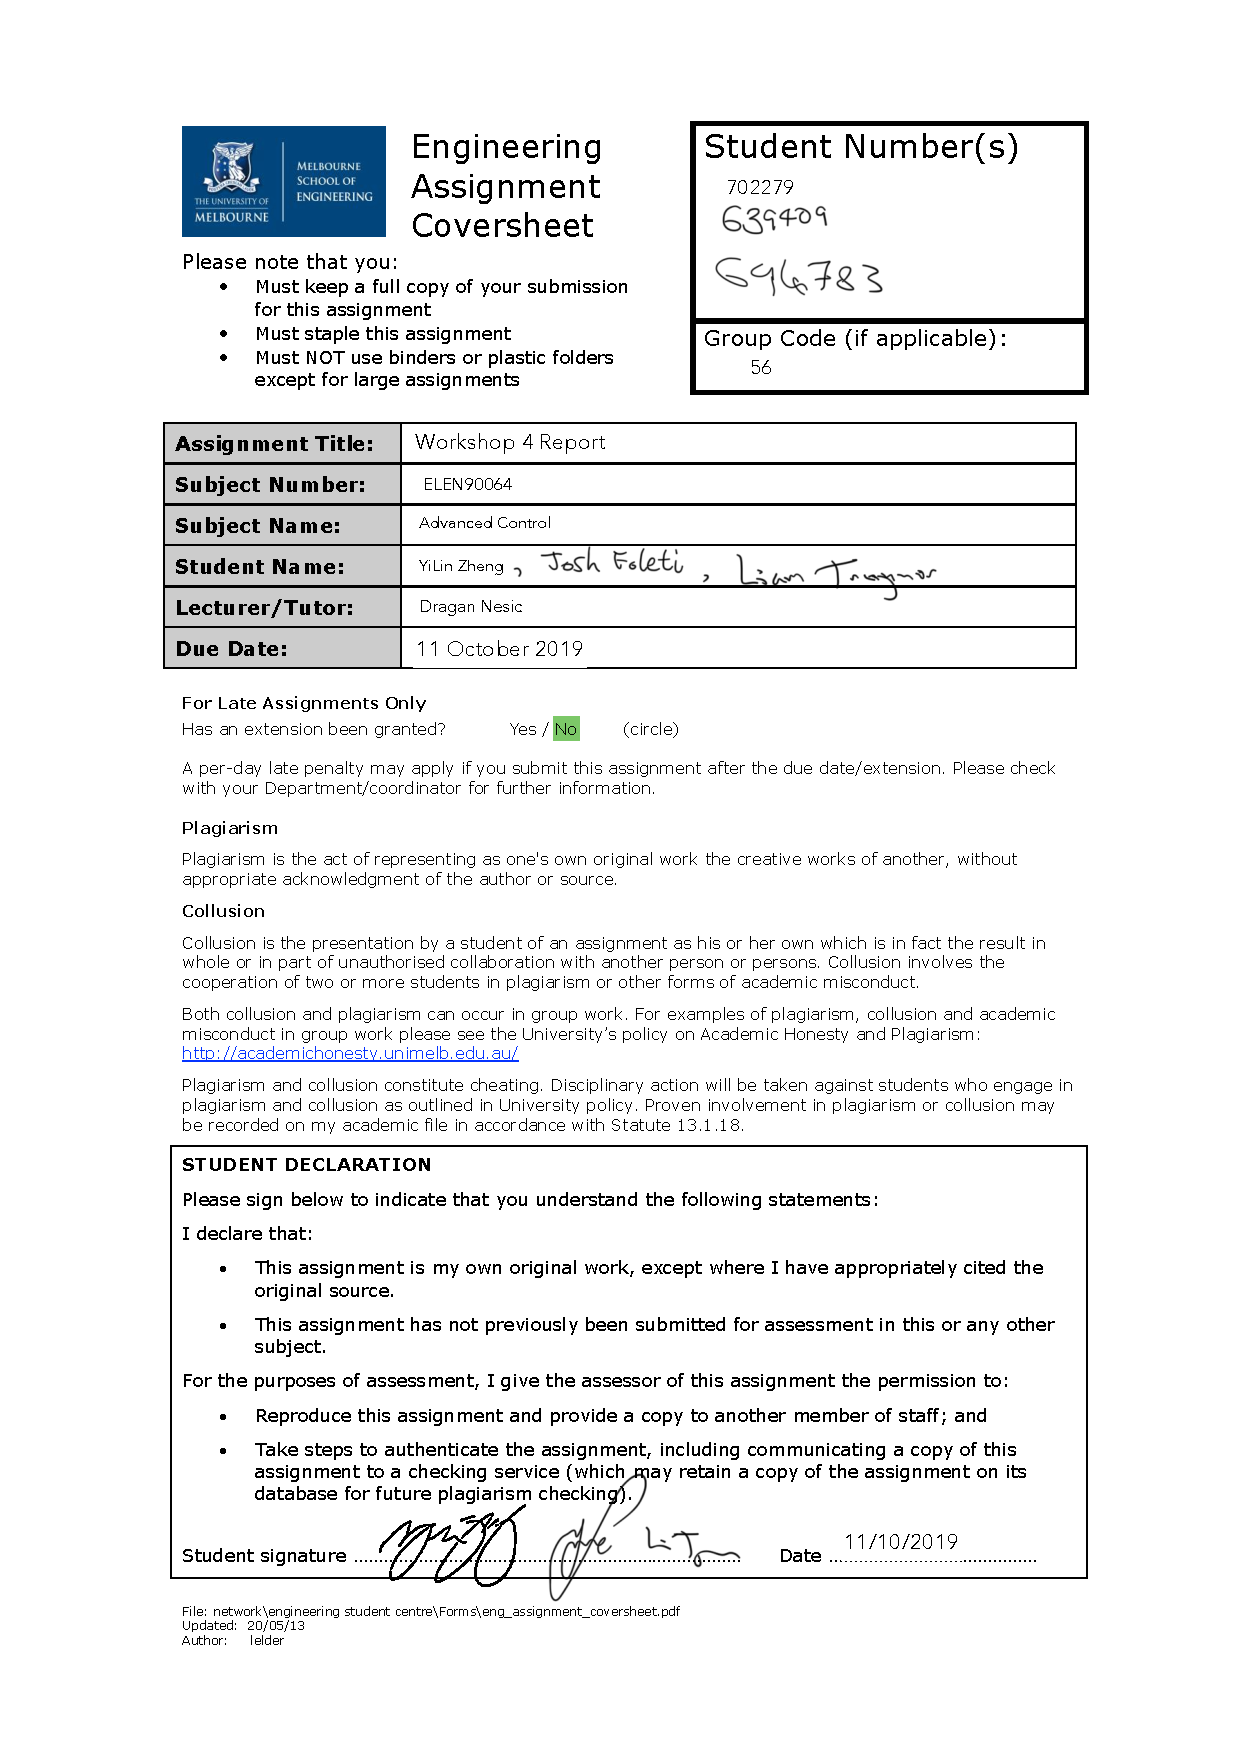
\includepdf{EngCSW4.pdf}
\clearpage
\setcounter{page}{1}

% Title
\begin{center}
\textbf{\Large{Modelling and PID Control for 2 DOF Configuration}}\\
Group 56: Josh Foleti [639409], Liam Traynor [694783], YiLin Inez Zheng [702279], \\
Workshop: Friday 1:00pm - 3:00pm Luis, Due: 11/10/19  
\end{center}

%%%%%%%%%%%%% BEGIN INTRODUCTION %%%%%%%%%%%%%%%%%
\section{Introduction}
The 2DOF Quanser Aero system can be abstracted into the axis arrangement shown in Figure \ref{fig:W4Quanser} with the navigation frame (fixed) denoted by $X$, $Y$, $Z$ and the body frame (varying) denoted by $X_B$, $Y_B$, $Z_B$. The pitch motor (0) rotates about $Y_B$ and increases in angle $\theta$ when moved upwards with a positive voltage $V_0$. The yaw motor (1) rotates about $Z$ and increases in angle $\psi$ when the body rotates counterclockwise with a positive voltage $V_1$.
\begin{figure}[H]
    \centering
    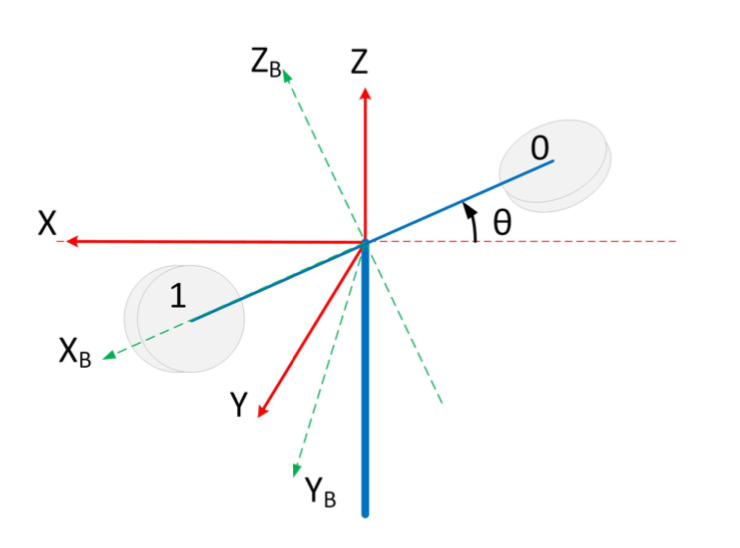
\includegraphics[width=6cm]{W4Quanser.png}
    \caption{Abstracted 2DOF Quanser Aero system}
    \label{fig:W4Quanser}
\end{figure}
In this workshop we aim to model the pitch and yaw axis of the Quanser Aero apparatus as a linearised 2DOF MIMO system. The two main objectives for this workshop are:
\begin{enumerate}
    \item To design PID controllers to stabilise the pitch and yaw axes at 10 and 45 degrees respectively.
    \item To design a controller and observer pair using the state space model for the 2DOF system.
\end{enumerate}

% Some description about what we did, steps for analysis and design
\subsection{Method}
The following are steps we followed in analysing and designing controllers/observers for our MIMO system.
\begin{enumerate}
    \item Experimentally determine system coefficients
    \item Linearise derived 2DOF system model
    \item Design and simulate PID controller for the linearised system against the following closed loop response specifications from Part 3 of the Quanser Aero Lab Guide:
    \begin{itemize}
        \item Steady state error: pitch $e_{ss} \leq 2^{\circ}$
        \item Peak time: $t_p \leq 2$seconds
        \item Percent overshoot: $PO \leq 7.5\%$
        \item No actuator saturation: $|V_y| \leq 24$V and $|V_p| \leq 24$V
    \end{itemize}
    \item Test PID controller on Quanser Aero
    \item Design and simulate controller/observer pair for the 2DOF state space system experimenting with both full and reduced state observers.
    \item Test controller/observer pair on Quanser Aero
\end{enumerate}

%%%%%%%%%%%% BEGIN SYSTEM MODELLING SECTION %%%%%%%%%%%%%%%%
\section{System Modelling and Analysis}
% Calculations and Simulation Results go here
\subsection{System Parameters}\label{section:coefficients}
% Empirical params
Table \ref{table:emp_params}, shows our experimental results.\\
\colorbox{yellow}{Enter descriptions on what the values mean etc.}
\begin{table}[H]
\begin{center}
\begin{tabular}{ |l|c|c|c| } 
    \hline
    \textbf{Parameter Attribute} & \textbf{Variable Name} & \textbf{Value} & \textbf{Unit} \\ 
    \hline
    \multirow{4}{4cm}{Thrust Torque Constant} 
    & $K_{pp}$ & 7.640882714810616$\cdot 10^{-4}$ & Nm/V\\ 
    & $K_{yy}$ & 0.003254390218108 & Nm/V\\ 
    & $K_{py}$ & 6.765292049137915$\cdot 10^{-4}$ & Nm/V\\
    & $K_{yp}$ & -0.001670223589461 & Nm/V\\
    \hline
    Stiffness & $K_{sp}$ & 0.041128897228432 & Nm/rad\\ 
    \hline
    \multirow{2}{4cm}{Viscous Damping} 
    & $D_{p}$ & 0.011277529550316 & Nms/rad\\ 
    & $D_{y}$ & 0.021186960335581 & Nms/rad\\ 
    \hline
\end{tabular}
\caption{Empirically determined parameters for the Quanser Aero system}\label{table:emp_params}
\end{center}
\end{table}
% Other params
Several system inertia values were calculated and the horizontal mass of the system was given via the Quanser Aero Lab Guide. Table \ref{table:calc_params} shows these parameters. 
\begin{table}[H]
\begin{center}
\begin{tabular}{ |l|c|c|c| } 
    \hline
    \textbf{Parameter Attribute} & \textbf{Variable Name} & \textbf{Value} & \textbf{Unit} \\ 
    \hline
    Horizontal body mass (Tube) & $M_b$ & 0.094 & kg\\ 
    \hline
    Moment of Inertia (Pitch) & $J_p$ & 0.0219 & kg$\text{m}^2$\\ 
    \hline
    Moment of Inertia (Pitch) & $J_y$ & 0.0220 & kg$\text{m}^2$\\ 
    \hline
\end{tabular}
\caption{Calculated and given parameters for the Quanser Aero system}
\label{table:calc_params}
\end{center}
\end{table}

\subsection{MIMO 2DOF System Linear Model}
The non-linear dynamics model of the Quanser Aero system can be derived via the Lagrangian equation in Eq \ref{eq:W4Lagrangian}, where $T$ is the total kinetic energy, $U$ is the total potential energy and $Q_i$ is the generalised forces along the system's independent coordinates $q_i$. 
\begin{equation*}\label{eq:W4Lagrangian}
    \frac{d}{dt}\frac{\partial T}{\partial \dot{q}_i} - \frac{\partial T}{\partial q_i} + \frac{\partial U}{\partial q_i} = Q_i
\end{equation*}

Following the Quanser Aero introduction in Figure \ref{fig:W4Quanser} we can set the center of mass $G$ coordinates $y_G$ and $z_G$ as a reference point for the independent coordinates used to solve Eq \ref{eq:W4Lagrangian}. The pitch and yaw axis are modelled as cylindrical solids turning about its respective axis. The overall non-linear model, expressed in terms of our parameter variables in Section \ref{section:coefficients}, is derived as Eq \ref{eq:W4nonlin1} and Eq \ref{eq:W4nonlin2}.
% Need to rewrite the equations using empirical parameters 
% and add note on Mb and g as parameters
\begin{equation}\label{eq:W4nonlin1}
    (M_b z^2_G + J_p)\ddot{\theta} + M_b g \sin \theta z_G - M_b\cos\theta y_G z_G \ddot{\psi} - M_b\sin \theta \cos\theta z^2_G \dot{\psi}^2 = K_{pp}V_0 + K_{py}V_1 - D_p \dot{\theta}
\end{equation}
\begin{equation}\label{eq:W4nonlin2}
    (M_b (y^2_G + \sin^2 \theta z^2_G) + J_y)\ddot{\psi} + 2M_b \sin \theta \cos \theta z^2_G \dot{\psi}\dot{\theta} - M_b\sin\theta y_G z_G \dot{\theta}^2 - M_b\cos\theta y_G z_G \ddot{\theta} = K_{yp}V_0 + K_{yy}V_1 - D_y \dot{\psi}
\end{equation}

When linearising around the equilibrium point $(\theta^{*}, \psi^{*}, \dot{\theta}^{*}, \dot{\psi}^{*}) = (0,0,0,0)$, we end up with Eq \ref{eq:ss_linear} as the state space model, where $\theta$ is the pitch angle (rad), $\psi$ is the yaw angle (rad), $\dot{\theta}$ is the pitch angular velocity (rad/s) and $\dot{\psi}$ is the yaw angular velocity (rad/s) for $\mathbf{x} = [\theta, \psi, \dot{\theta}, \dot{\psi}]^{T}$, $\mathbf{y} = [\theta, \psi]^T$, and $V_0$ is the pitch motor voltage input, $V_1$ is the yaw motor voltage input for $\mathbf{u} = [V_0, V_1]^T$. \textit{See detailed calculations in Appendix \ref{app:linearise}}
\begin{equation}\label{eq:ss_linear}
\begin{array}{ccc}
    \mathbf{\dot{x}} = \mathbf{A}\mathbf{x} + \mathbf{B}\mathbf{u}
    \\
    \mathbf{y} = \mathbf{C}\mathbf{x} + \mathbf{D}\mathbf{u}
\end{array}
\end{equation}
\begin{align*}
\mathbf{A} &= \begin{bmatrix}
    0 & 0 & 1 & 0\\
    0 & 0 & 0 & 1\\
    \frac{(M_b y^2_G + J_y)M_b g z_G}{(M_b y_G  z_G)^2 - (M_b z^2_G + J_p)(M_b y^2_G + J_y)} & 0 & \frac{(M_b y^2_G + J_y) D_p}{(M_b y_G  z_G)^2 - (M_b z^2_G + J_p)(M_b y^2_G + J_y)} & \frac{M_b y_G  z_G D_y}{(M_b y_G  z_G)^2 - (M_b z^2_G + J_p)(M_b y^2_G + J_y)}\\
    \frac{M^2_b g y_G z^2_G}{(M_b y_G  z_G)^2 - (M_b z^2_G + J_p)(M_b y^2_G + J_y)} & 0 & \frac{M_b y_G  z_G D_p}{(M_b y_G  z_G)^2 - (M_b z^2_G + J_p)(M_b y^2_G + J_y)} & \frac{(M_b z^2_G + J_p) D_y}{(M_b y_G  z_G)^2 - (M_b z^2_G + J_p)(M_b y^2_G + J_y)}
    \end{bmatrix}\\
\mathbf{B} &= \begin{bmatrix}
    0 & 0\\
    0 & 0\\
    -\frac{M_b y_G  z_G K_{yp} + (M_b y^2_G + J_y) K_{pp}}{(M_b y_G  z_G)^2 - (M_b z^2_G + J_p)(M_b y^2_G + J_y)} & -\frac{M_b y_G  z_G K_{yy} + (M_b y^2_G + J_y) K_{py}}{(M_b y_G  z_G)^2 - (M_b z^2_G + J_p)(M_b y^2_G + J_y)}\\
    -\frac{(M_b z^2_G + J_p) K_{yp} + M_b y_G  z_G K_{pp}}{(M_b y_G  z_G)^2 - (M_b z^2_G + J_p)(M_b y^2_G + J_y)} & -\frac{(M_b z^2_G + J_p) K_{yy} + M_b y_G  z_G K_{py}}{(M_b y_G  z_G)^2 - (M_b z^2_G + J_p)(M_b y^2_G + J_y)}
    \end{bmatrix}\\
\mathbf{C} &= \begin{bmatrix}
    1 & 0 & 0 & 0\\
    0 & 1 & 0 & 0
    \end{bmatrix} \hspace{1cm}
\mathbf{D} = \begin{bmatrix}
    0 & 0\\
    0 & 0
\end{bmatrix}
\end{align*}

Setting the centre of gravity $G$ coordinates, $y_G = z_G = 0$ as the reference point for the Quanser Aero body, this simplifies the above state space matrices to the system below, where it resembles the mechanically derived system from the lab guide,
\begin{align*}
\mathbf{A} = \begin{bmatrix}
    0 & 0 & 1 & 0\\
    0 & 0 & 0 & 1\\
    0 & 0 & -\frac{D_p}{J_p} & 0\\
    0 & 0 & 0 & -\frac{D_y}{J_y}
    \end{bmatrix} \hspace{1cm}
\mathbf{B} = \begin{bmatrix}
    0 & 0\\
    0 & 0\\
    \frac{K_{pp}}{J_p} & \frac{K_{py}}{J_p}\\
    \frac{K_{yp}}{J_y} & \frac{K_{yy}}{J_y}
    \end{bmatrix} \hspace{1cm}
\mathbf{C} = \begin{bmatrix}
    1 & 0 & 0 & 0\\
    0 & 1 & 0 & 0
    \end{bmatrix} \hspace{1cm}
\mathbf{D} = \begin{bmatrix}
    0 & 0\\
    0 & 0
\end{bmatrix}
\end{align*}

We see that the matrices above ignored the stiffness coefficient $K_{sp}$. This is a key component to model a more realistic mechanical system as we found out in primary runs that the system would settle with a small steady state error $e_{ss}$ due to its stiffness properties. We therefore added this to our system following the Quanser Aero Lab Guide as $\mathbf{A}(3,1) = -\frac{K_{sp}}{J_p}$. The model we use to simulate the 2DOF system hence matches with that in the lab guide.\\

Substituting our empirical parameters in Section \ref{section:coefficients}, the linearised state space model now has the state matrices, where gravity $g = 9.81\text{ms}^{-2}$,
\begin{align*}
\mathbf{A} = \begin{bmatrix}
    0 & 0 & 1 & 0\\
    0 & 0 & 0 & 1\\
    -1.8792 & 0 & -0.5153 & 0\\
    0 & 0 & 0 & -0.9634
    \end{bmatrix} \hspace{.5cm}
\mathbf{B} = \begin{bmatrix}
    0 & 0\\
    0 & 0\\
    0.0349 & 0.0309\\
    -0.0759 & 0.1480
    \end{bmatrix} \hspace{.5cm}
\mathbf{C} = \begin{bmatrix}
    1 & 0 & 0 & 0\\
    0 & 1 & 0 & 0
    \end{bmatrix} \hspace{.5cm}
\mathbf{D} = \begin{bmatrix}
    0 & 0\\
    0 & 0
\end{bmatrix}
\end{align*}

\subsection{System Analysis}
\colorbox{yellow}{Enter in observability/controllabiity calcs, Kalman decomp stuff}

\newpage
\section{PID Controller} %%%%% PID %%%%%%%%%%

\subsection{PID Design and Simulation}
A decoupling approach was used in designing the PID controllers so that the pitch and yaw motor input voltages are controlled separately. For this part we followed the Quanser Aero Lab Guide in implementing a modified PID controller, where only the negative voltage is used in feedback and a derivative term (acting as a high pass filter) is used to suppress measurement noise. In essence we aimed to design a proportional velocity (PV) controller with added integration $K_i$.\\ 

We used the transfer functions for the respective outputs pitch and yaw angles with respect to pitch and yaw motor input voltages to simulate the PID controllers. They are Eq \ref{eq:PitchVp}-\ref{eq:YawVy} below.
\begin{equation}\label{eq:PitchVp}
    \frac{\Theta (s)}{\text{V}_0 (s)} = \frac{0.03491}{s^2 + 0.5153 s + 1.879}
\end{equation}
\begin{equation}\label{eq:PitchVy}
    \frac{\Theta (s)}{\text{V}_1 (s)} = \frac{-0.07595}{s^2 + 0.9634 s - 6.473\cdot 10^{-17}}
\end{equation}
\begin{equation}\label{eq:YawVp}
    \frac{\Psi (s)}{\text{V}_0 (s)} = \frac{0.03091}{s^2 + 0.5153 s + 1.879}
\end{equation}
\begin{equation}\label{eq:YawVy}
    \frac{\Psi (s)}{\text{V}_1 (s)} = \frac{0.03491}{s^2 + 0.9634 s - 6.473\cdot 10^{-17}}
\end{equation}
Percentage overshoot $PO$ and peak time $t_p$ in the second order transfer function can be derived to have the following system responses below, where $PO$ is inversely proportional to the damping coefficient $\zeta$, and $t_p$ is inversely proportional to both $\zeta$ and the natural frequency $\omega_n$. This indicates that $PO$ influences the smoothness and steady state value of the response and $t_p$ influences the speed of the response as well as system oscillations.
\begin{align*}
    PO &= 100 e^{-\frac{\pi \zeta}{\sqrt{1 - \zeta^2}}}\\
    t_p &= \frac{\pi}{\sqrt{1 - \zeta^2}}
\end{align*}
Starting at our maximum specification of percentage overshoot $PO = 7.5$\% and peak time $t_p = 2$s, we first gradually reduced $t_p$ to reduce the oscillations in the response to hit a relatively steady state. Then we reduced $PO$ to reduce the steady state error $e_{ss}$. Figures X-Y show the results of our simulations.\\ \textit{See Appendix Section X for the Simulink model.}

\subsection{PID Quanser Aero Implementation}

%%%%%%%%%%%% Controller/Observer %%%%%%%%%%%%%%%%
\newpage
\section{Controller/Observer Pair Design}
% Design 

\subsection{Full State Feedback Controller Design and Simulation}
%LQR simulations 

\subsection{Observer Design}

\subsubsection{Full State Observer}

\subsubsection{Reduced State Observer}

\section{Controller/Observer Pair Quanser Aero Implementation}
\subsection{Full State Feedback Controller Implementation}
% Quanser

\subsection{Quanser Aero Observer Implementation}

\subsubsection{Full State Observer}

\subsubsection{Reduced State Observer}

%%%%%%%%%%%% BEGIN CONCLUSION %%%%%%%%%%%%%%%%
\section{Conclusions}
\colorbox{yellow}{Thought ramble below about discussion points:}\\
\textcolor{blue}{• Dynamic system is inadequately modelled. Yaw and pitch inertia values are insufficiently calculated\\
• Modelled mass values as point masses not solids and ignores aerodynamics of rotor shape, \\hence heavy/"un"controllable spikes in pitch when yaw changes vice versa\\
• Decoupled yaw and pitch control in PID vs FSF controllers\\
• Center of gravity $G$ modelling?\\
• The mass of the entire apparatus considered as a spoke?}\\

\textcolor{red}{
• Linearized model of 2DOF configuration for zero equilibrium state (all equilibrium values are zero).\\
• An identified model of 2DOF configuration for Quanser Aero; please include all exper- iments and calculations of all parameters for the model.\\
• Design of PID controllers for the pitch and yaw axes for the derived 2DOF model using the design specifications given in Section 3 of [1]; note that your controller should contain some integral action and so you can not simply rely on [1] where only PD controllers are designed. Please include all design steps, simulations of the closed-loop model and the experiments on the real closed-loop system.\\
• Derivation of the state-space model for 2DOF model, a complete analysis of your 2DOF as per the above instructions; and the design, simulation, and implementation of the state space controller/observer pair.}

\newpage
\section{Appendix}
\subsection{Linearisation of 2DOF Quanser Aero Model}\label{app:linearise}

\end{document}
